	%import packages%
\documentclass[12pt]{article}
\usepackage[a4paper]{geometry}
\usepackage[myheadings]{fullpage}
\usepackage{fancyhdr}
\usepackage{lastpage}
\usepackage{wrapfig, subcaption, setspace, booktabs}
\usepackage[T1]{fontenc}
\usepackage[font=small, labelfont=bf]{caption}
\usepackage{fourier}
\usepackage[protrusion=true, expansion=true]{microtype}
\usepackage[utf8]{inputenc}
\usepackage[francais]{babel}
\usepackage{sectsty}
\usepackage{url, lipsum}
\usepackage{tgbonum}
\usepackage{hyperref}
\usepackage{xcolor}
\usepackage{graphicx}
\usepackage[none]{hyphenat}
\usepackage{endnotes}
\renewcommand{\footnote}[1]{\endnote{#1}}
\renewcommand{\theendnote}{}
\let\cleardoublepage\clearpage
\newcommand{\HRule}[1]{\rule{\linewidth}{#1}}
\onehalfspacing
\setcounter{tocdepth}{5}
\setcounter{secnumdepth}{5}



	%page de couverture%
\begin{document}
\begin{figure}[t]
	
\includegraphics[width=4cm]{./images/logoesiee.png}
	\hfill
	
\includegraphics[width=4cm]{./images/cnrs.png}	
\end{figure}

\fontfamily{cmr} \selectfont
\title{ \normalsize \textsc{}
	\\ [2.0cm]
	\HRule{0.5pt} \\
	\LARGE \textbf{\uppercase{Rapport de stage}
	\HRule{2pt} \\ [0.5cm]
	\normalsize  \vspace*{5\baselineskip}}
}

\date{Du 1 au 26 Juillet 2019}

\author{
	Théo PERESSE-GOURBIL\\ 
	ESIEE Paris \\
	Rapport de stage de fin de E1 }
\maketitle


\newpage
\section{Introduction}
Afin de clôturer la première année à l'ESIEE Paris, chaque élève doit effectuer un stage d'exécution d'une durée de 4 semaines en entreprise. Ce stage d’exécution permet à l’élève d’avoir un premier contact avec la vie active. 
J'ai choisis d'effectuer ce stage dans le domaine de l'informatique. En effet, cela correspond à mes envies actuelles d'orientation pour mes futures années à l'ESIEE. Ma mère travaillant au CNRS, j'ai pu obtenir le contact de Mr Etienne FAURE, responsable du pôle SI de l'IFSeM\footnotemark, pôle que je détaillerais plus tard. J'ai donc envoyé à Mr Faure une lettre de motivation et un Curriculum Vitae. A la suite d'un entretient téléphonique, il a accepté de me prendre comme stagiaire du 1er au 26 juillet 2019. 
\footnotetext{Ile-de-France Service Mutualisé}
L'IFSeM est situé au 7 rue Guy Moquet, à Villejuif. Je travaillais du lundi au vendredi, entre 9h et 17h42, avec donc une amplitude horaire de 7h42 par jours. Cette amplitude n'était pas fixe. En effet, certains jours on me demandait d'arriver plus tôt, ou plus tard. 
\medbreak
L'activité sur le campus n'était pas très importante. En effet, mon stage pendant le mois de juillet tombait sur une période durant laquelle de nombreux agents étaient en vacances. De plus, au vu des très fortes chaleur caniculaires qui ont eus lieu, bon nombre d'employés travaillaient depuis chez eux, ce qui ne m'étais pas permis. Sur le campus était présent une cantine. C'est un gros point fort pour la restauration.
\medbreak
Dans ce rapport, je parlerais dans un premier temps de l'entreprise, plus particulièrement du service où j'ai effectué mon stage : le SI de l'IFSeM. Ensuite, je parlerais du travail et des taches qui m'ont été confiées durant ce stage, puis du résultat que j'en ai tiré au point de vu personnel et professionnel. 
\newpage

\tableofcontents
\smallbreak 
% \vspace{1\baselineskip}



\newpage

\sectionfont{\scshape}

	%pages de texte%
	
\section{Présentation et fonctionnement de l'entreprise}
\subsection{Présentation du CNRS}
Le CNRS, ou Centre National de la Recherche Scientifique, est une institution de recherche parmi les plus importantes au monde. Pour relever les grands défis présents et à venir, ses scientifiques explorent le vivant, la matière, l’Univers et le fonctionnement des sociétés humaines. Mondialement reconnu pour l’excellence de ses travaux scientifiques, le CNRS est une référence, aussi bien dans l’univers de la recherche et du développement, que pour le grand public. Le CNRS étant une importante entreprise publique, les domaines de recherches sont très vastes (sciences, langues, histoires, mathématiques \ldots). 

\subsection{Présentation de l'IFSeM}
\textit{"Créé en juillet 2015, le Service Mutualisé d’Île-de-France, rattaché à la Délégation Paris-Villejuif, prend en charge des activités jusqu’alors exercées par les 5 délégations franciliennes et les regroupe en 4 pôles de compétences au bénéfice de toutes\footnotemark. "}
\footnotetext{https://www.dr1.cnrs.fr/spip.php?rubrique59}
\smallbreak
Voici ce que l'on peut lire sur le site de la délégation Ile-de-France-Villejuif du CNRS. Comme expliqué en introduction, l'IFSeM est situé à Villejuif, sur le même campus que la délégation régionale numéro 1 (DR01). L'IFSeM est constitué de 4 pôles : Formation, Achats, Système d'information et Patrimoine immobilier. Ces pôles ont pour mission de "gagner en cohérence et permettre à toutes les délégations d'Ile-de-France d’apporter le meilleur niveau de service à ses unités comme à son personnel".

\subsection{Présentation du pôle SI de l'IFSEM}
J'ai donc choisi, dans la continuité de mon projet à ESIEE Paris, d'effectuer ce stage d'un mois au pôle informatique de l'IFSeM, dans l'équipe infrastructure. 
Ce pôle a pour objectif d'apporter une assistance technique à 4 délégations différentes du CNRS : la DR01, située à Villejuif, la DR02, à Paris-Centre, la DR04 à Gif-Sur-Yvettes et la DR05 située à Meudon. De plus, ce service a pour but de maintenir et mettre à jour les applications nationales du CNRS au travers de différents serveurs décentralisés. 
\newpage
\subsection{Fonctionnement de l'entreprise : Le travail en équipe}

Le pôle informatique de l'IFSeM est divisé en 3 équipes (pour l'organigramme complet, se reporter, en annexe, au point 5.1.1) : 
\begin{itemize}
    \item Le support aux applications et offre de services : \textit{"support et exploitation de la téléphonie IP après déploiement, support des applications nationales du CNRS, création et accompagnement de la mise en oeuvre de l’offre de services nationale pour les délégations concernées et les laboratoires qui en dépendent.\footnotemark[3]"}
    \item La gestion des infrastructures : \textit{"gestion de parc informatique, sécurité informatique (communication/formation à destination des unités, support à la gestion des incidents), et gestion des systèmes et réseaux (support à l’ingénierie, gestion propre au Service Mutualisé, supervision des raccordements de sites).\footnotemark[3]"}
    \item Le développement logiciel : \textit{"besoins applicatifs propres au Service Mutualisé et applications métiers recouvrant les besoins communs aux 5 délégations.\footnotemark[3]"}
\end{itemize}
\footnotetext[3]{Voir note 2}
\smallbreak
Durant mon stage, j'ai été affecté à l'équipe "Gestion des infrastructures". J'étais dans un bureau de 4 personnes. J'ai pu observer que les trois équipes collaboraient au travers d'échanges et de discussions, et chacun apportait son aide et participait à la recherche de solutions des autres groupes. 
Ces trois équipes sont sous la direction de Mr Etienne FAURE, Ingénieur de Recherches.

\subsubsection{Le ticketing}
Une machine virtuelle faisant tourner un serveur OTRS (Open-source Ticket Request System) permet aux utilisateurs qui rencontrent un problème de le notifier au travers d'un ticket d'assistance aux 3 équipes du SI. \\
Le ticketing est la méthodologie qui est employée pour la résolutions des faits techniques remontés par les utilisateurs :
\begin{itemize}
    \item L'utilisateur ouvre un ticket depuis un site internet
    \item En fonction du type de problème, l'équipe concerné (support, infra ou dev) prend en charge le ticket.
    \item Si le problème concerne un seul utilisateur, une fois résolu, le ticket est fermé.
    \item Si le problème concerne plusieurs utilisateurs, on applique des GPO (Group Policy Object). C'est un ensemble de règles qui sont appliquées de différentes façons (à tous les ordinateurs, tous les utilisateurs, un groupe, une seule personne, un service ...). C'est ce que l'on appelle une stratégie de groupe. Cela permet de corriger le problème pour tout le monde, et non au cas par cas.
\end{itemize}
Dès l'instant où le ticket est pris en charge, il disparaît de l'écran des autres membres du SI, afin de faciliter son traitement et d'éviter les doublons, ce qui ferait perdre beaucoup de temps. Cela n'empêche en rien les autres équipes d'apporter leur aide à la personne qui a bloqué le ticket. En effet, toutes les personnes ayant lu le message sont au courant du problème et peuvent apporter leur aide.\\
\vspace{2\baselineskip}
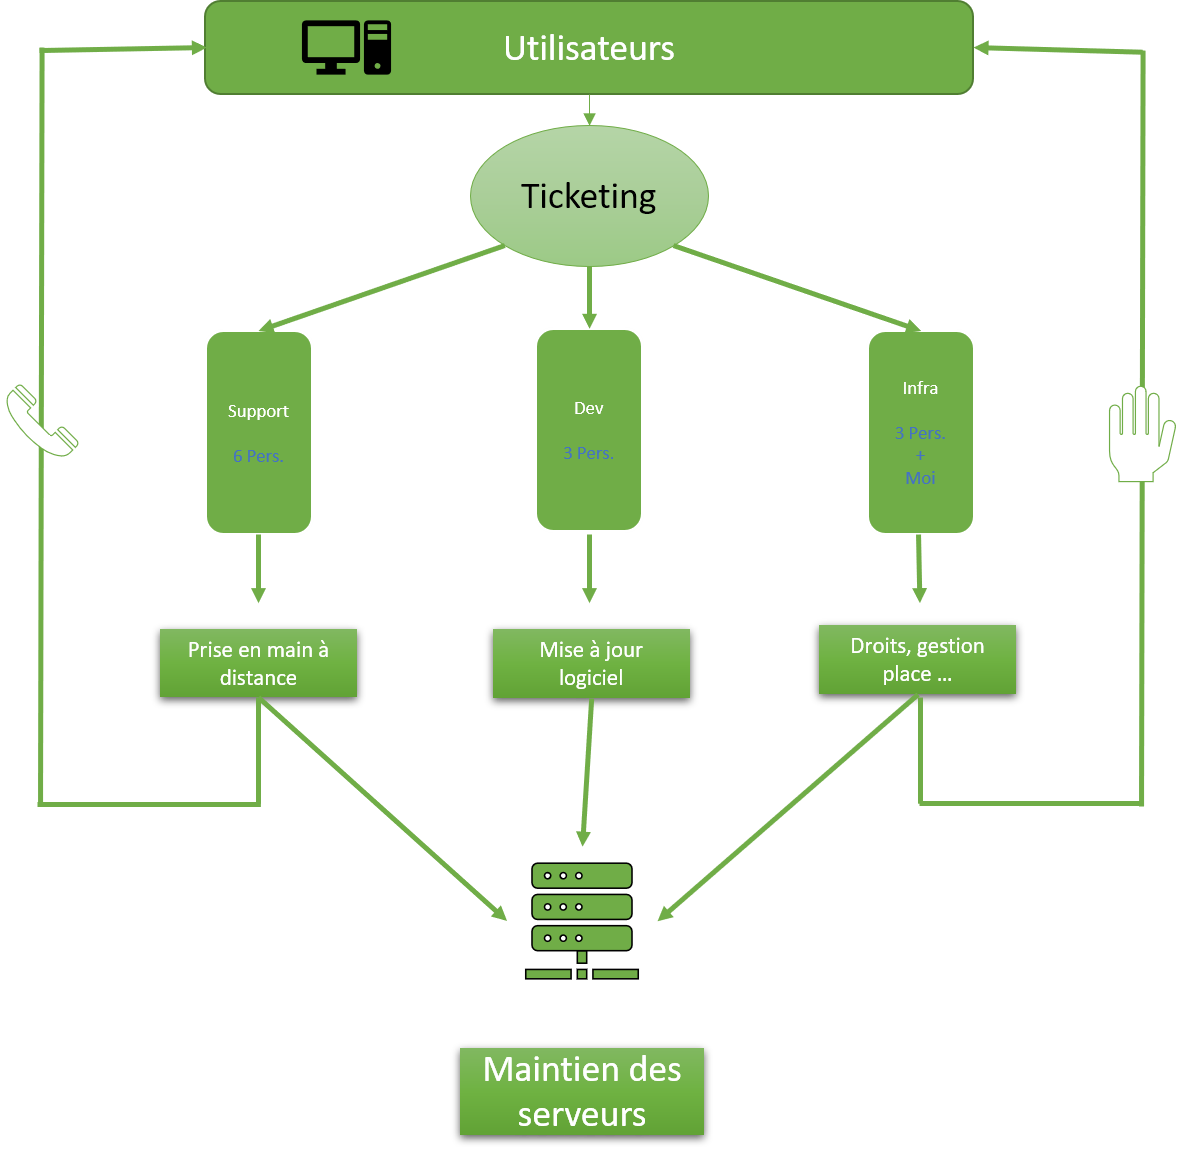
\includegraphics[width=15cm]{./images/orga.png}
\newpage

\subsubsection{Coordination intra-équipe}
La coordination intra-équipe est facile et naturelle. En effet, les bureaux sont composés d'un petit nombre de personne, mais toujours 2 au minimum. De plus, les équipes sont assez restreintes, entre 3 et 6 personnes au maximum pour l'équipe support. La communication se fait donc naturellement. Lorsqu'un membre d'une équipe a un problème, une demande ou une information à faire passer, il peut simplement en parler avec les autres membres de son équipes. 
De plus, les bureaux étant occupés par des membres d'une même équipe, cela facilite les échanges, et on peut parler assez fort sans risquer de gêner les autres équipes qui sont dans des bureaux différents. 

\subsubsection{Coordination inter-équipe}
De par la séparation des bureaux évoquée au paragraphe précédent, il à été mis en place des réunions de service, regroupant une partie ou l'entièreté du pôle SI, afin de d'échanger sur des sujets communs. \\
Un exemple de réunion à laquelle j'ai assisté est la réunion mensuelle organisée par Baptiste BARAKOWSKY, responsable de l'équipe "Gestion des infrastructures", afin d'expliciter les différents GPO qui sont appliquées par l'IFSeM. En effet, plus le nombre de problème augmente, plus le nombre de GPO est important. Cette réunion à donc pour but d'informer les autres équipes des correctifs qui sont déjà appliqués.

\subsubsection{Des échanges informels au service du groupe}
La communication et la cohésion de groupe étant primordiale dans ce genre d'organisation, la "pause café" se révèle constructive au sein d'un groupe comme celui-là. En effet, selon les statistiques, 84\% des salariés jugent important d'avoir une machine à café à disposition dans les locaux de l'entreprise. Cela permet de développer la solidarité entre les membres des différentes équipes, en plus d'être un lieu de détente et d'échanges.
\smallbreak
Dans le cas de l'IFSeM, ces pauses permettait un échange entre les différentes équipes, et même avec les différents pôles de l'IFSeM. Cela permet aux personnels d'échanger, aussi bien sur le plan professionnel que personnel. 
Ces pauses permettent une bonne ambiance de travail et une certaine complicité entre les membres des différentes équipes, qui ne peut qu'être bénéfique au service. En effet, si les personnes s'entendent bien entre elles, le dialogue en est facilité.  

\subsubsection{Moyens de communications internes}
Le CNRS, comme de nombreuses organisations de cette taille, dispose de différents moyens de communications qui sont plus ou moins utilisés :
\begin{itemize}
    \item Le téléphone : chaque agent dispose d'un téléphone IP dans son bureau. Dans le cas du SI, ce téléphone sert uniquement à communiquer avec les utilisateurs qui ont besoin d'aide;
    \item Les mails : l'envoi de mails est soit officiel (administratifs, échanges avec l'extérieur du CNRS\dots) soit interne. Dans ce cas, les mails servent principalement pour garder une trace écrite sans encombrer le disque dur, soit pour transférer des documents (Word par exemple).
    \item La messagerie instantanée : l'utilisation de messagerie instantanées permet aux employés de créer des groupes, de discuter, d'envoyer des informations, de poser des questions\dots depuis leurs bureaux respectifs. Cela permet premièrement de gagner du temps, par rapport aux mails par exemple, mais aussi d'être plus multi-tâche. En effet, on peut très bien parler au téléphone avec un utilisateur et poser une question à un autre membre de l'équipe, sans pour autant être gêné dans son travail.
\end{itemize}
\newpage


\section{Travail effectué}
\subsection{Hotline et assistance aux utilisateurs : MCO-Windows}
Une importante partie du travail consistait en l'aide aux utilisateurs. De ce fait, en plus du système de ticketing évoqué plus haut, le pôle SI faisait aussi office de centre hotline pour les utilisateurs. Tous les membres disposaient d'un téléphone fonctionnant pat téléphonie IP, permettant d'appeler n'importe quel agent du CNRS.

\subsubsection{L'infogérance}
Une fois que le problème est identifié (appel ou ticket), une phase de recherche commence. La première chose à verifier est si ce problème à déjà été reporté et/ou si un problème proche à déjà été corrigé dans le passé. Si c'est le cas, il faudra alors appliqué une GPO. Une GPO est une règle que l'on peut appliqué à différents niveau. Tout cela demande une grande organisation. 
\medbreak
\textit{Un exemple concret que j'ai rencontré lors de mon stage est un problème qui survient lorsqu'une machine uniquement de la marque Hewlett-Packard Company (HP) se connecte à un VPN. Un processus en fond détectait la connexion VPN comme étant une connexion filaire et désactivait donc automatiquement le Wifi, ayant pour effet de couper la connexion avec le VPN. Cette personne ne pouvait don pas travailler de chez elles, car l'ensemble des application nationales ne sont accessibles que depuis l'intérieur du cnrs, donc soit physiquement soit au travers d'un VPN. La solution consistait donc à arrêter ce processus dès le démarrage de toutes les machines HP.}
\medbreak
En plus des GPO qui régissent le parc informatique, l'IFSeM dispose d'un serveur Dell, appelé K1000, permettant de gérer l'ensemble du parc informatique. Ce serveur permet de savoir exactement qui s'est connecté sur quelle machine, à quelle heure, qui est connecté en temps réel\dots De plus, cela permet de gerer les mises à jour système et logiciel pour tout le monde. Le but étant qu'un utilisateur ne se rendent compte de rien. Les mises à jour sont donc éfféctuées avec des options qui les rendent silencieuse, les grosses maj sont efféctuées de nuit\dots 

\newpage

\subsubsection{Déploiement de l'image IFSeM}
En informatique, on parle d'image système ou image, un système d'exploitation (dans notre cas un système Windows 10 Pro que l'on va deployer en grand nombre. On peut stocker une image sur un CD (comme les CD d'installation Windows), une clé USB ou encore accessible sur un serveur depuis le réseau (cas du CNRS) à l'aide du protocole PXE. 
\medbreak
Lorsqu'une nouvelle machine (portable ou fixe) était livré, il fallait déployer dessus l'image standard crée par l'IFSeM. En effet, jusqu'à présent, chaque délégation possédait sa propre image, que le SSI local (service système d'information, chaque délégation dispose d'un SSI local) déployait sur chaque machine qu'ils recevaient. Cependant, depuis quelques mois, il a été décidé de déployer une image unique sur tous les postes de chaque délégation, afin de faciliter le travail et la gestion à distance du parc informatique.
\medbreak
J'ai donc du me déplacer, avec l'équipe Gestion des Infrastructures sur le site de Meudon, afin de déployer des images systèmes et installer les postes qui venaient d'être livrés. Cela permet de mieux gérer l'infrastructure de l'ensemble des postes (En annexe l'ordre de mission confirmé par le service des stages). Cette intervention sur un autre site que celui de Villejuif m'a permis de découvrir un autre environnement de travail et de me rendre compte des difficultés des interventions sur un autre site. En effet, en plus des problèmes réseaux, nous avons du attendre que le matériel demandé arrive car il n'avait pas été préparé en amont par le SSI local. 

\subsection{Maintien des applications nationales : MCO-Linux}
Une des grosses parties du travail que j'ai effectué durant ce stage fut du MCO-Linux. MCO, ou Maintient en condition opérationnelles consiste à assurer une continuité de service et une disponibilité des services hébergés sur les hyperviseurs. \\
La plupart des services sont hébergés sur des hyperviseurs, eux même divisés en plusieurs machines virtuelles. Il faut alors impérativement garantir une accessibilité à ces services. Lors d'un bug, nous devions alors basculer sur le serveur de secours, afin que les utilisateurs ne se rendent pas compte du bug, puis de corriger ce dernier. Cette tache dépendait alors complètement du type de service et du type de bug. Le plus souvent, un simple reboot de la VM (Virtual-Machine), l'observation des logs (journaux tenus à jour par la machine), ou même une restauration à une version antérieure suffisait à résoudre le bug. 

\subsubsection{Sauvegardes des machines virtuelles}
L'IFSeM disposait d'un serveur de stockage (10 To ) permettant de stocker les sauvegardes des différentes applications. Ce serveur (qui est en réalité une VM), fait tourner l'application BackUpPC, une application avec une interface web permettant de gerer les sauvegardes de toutes les VM. La place étant limité, un système de roulement des sauvegardes est mis en place automatiquement par BackUpPC, afin de ne garder que certaines sauvegardes (partielles et totales). \\
Une des tâches que j'ai effectué fut de mettre en place un planning des sauvegardes. Une autre tache que j'ai du effectuer fût d'augmenter la place du serveur de sauvegarde. En effet, plus le temps passe, plus les sauvegardes sont lourdes. Il est donc arrivé à un point où le serveur était plein. On a donc sollicité mon aide afin d'augmenter la taille de la partition du disque virtuelle accessible depuis la VM, sans pour autant écraser les sauvegardes. Après avoir, pendant une journée, reproduis la situation sur un environnement de test, j'ai réussi sans encombre l'agrandissement de la partition, qui est une opération qui peut s'avérer périlleuse, surtout que seule les outils en ligne de commande étaient disponible : Parted, resize ...

\subsection{La documentation}
Une grand partie de mon travail durant ce stage fut de compléter la documentation. En effet, chacun des pôles cités dans 1.3 possédaient leur propre documentation personnel, souvent au format Word ou même bloc-note. Un projet en cours lors de mon arrivé était de regrouper toutes les docs sur un Wiki accessible par tout l'IFSeM. J'ai donc du recopier et transférer les documents depuis les fichiers world vers le Wiki. \\
De plus, afin de vérifier que les informations étaient corrects, il m'a été demandé de suivre et de réaliser le contenu de ces documentations et de prendre des captures d'écran des messages affichés. 
Ce travail m'a pris environ 50\% de mon temps. Bien que peut intéressante, cette tâche est pourtant nécessaire et permet aux employés de gagner beaucoup de temps. 
\newpage

\section{Bilan personnel et professionnel : \\  Secteur d'activité}
\subsection{L'informatique}
Ma passion pour l'informatique m'a fait me tourner vers un stage en lien avec le réseau et les systèmes d'informations. 
Ce stage fut pour moi l'occasion de découvrir un métier qui pourrait s'apparenter à Administrateur Réseau ou Administrateur système. Cela m'a permis de confirmer mon choix d'orientation. J'ai pris par exemple énormément de plaisir à sécuriser des serveurs des attaques extérieurs (changement de ports, cloisonnement, Fail2Ban\dots). Ce stage m'a permis de comprendre et de me rendre compte des techniques et méthodes utilisées dans un grand établissement comme le CNRS. En effet, dans ce type de grandes entreprises, la gestion du parc informatique, de son maintien et de ses mises à niveau nécessite une organisation et des méthodes qui s’avèrent complexes.

Par exemple, il ne suffit pas de brancher une machine à une prise réseau (RJ45) pour qu'elle soit connectée. En effet, afin de limiter les accès réseau et les risques d'intrusions informatiques, il faut au préalable demander l'enregistrement de la machine dans le serveur DHCP afin qu'elle soit connectée. Comprendre le fonctionnement du réseau informatique m'a vraiment plu. De plus, le réseau d'un établissement aussi important que le CNRS ne peut pas être parfait. Il y a toujours du travail afin d'améliorer l'expérience des utilisateurs (vitesse de connection, sécurité,\ldots).
\medbreak
Je me suis rendu compte que l'on ne peut pas faire ce que l'on veut sur les serveurs. En effet, on passe systématiquement par une phase de tests dans un environnement sûr afin de limiter les risques. Il faut alors comprendre le lien entre les différentes machines (lien réseau principalement), avant de reproduire une maquette de ces serveurs afin de tester ce que l'on veut faire. Cela nécessite une certaine rigueur car le bon fonctionnement de l'établissement dépend de nos actions.
\medbreak
En revanche, une partie qui me passionne moins dans l'informatique est le développement logiciel. En effet, les développements que j'ai eu à effectuer (PowerShell et shell) me sont apparus bien moins passionnant et intéressant, en particulier si le code était long. Un petit script de quelques lignes ne me posait pas problème, mais de longs projets me paraissaient moins attirants. 
\medbreak
Ce stage m'a permis de confirmer mon souhait d'orientation vers l'informatique. J'ai donc pu écarter la partie développement pour les raisons citées ci-dessus. Je pense donc choisir une filière tournée vers la cybersécurité ou le réseau. 
 
\subsection{Hotline et assistance}
J'ai trouvé très délicat d'échanger avec des personnes non initiées en informatique. En effet, les personnels qui venaient nous voir étaient souvent très énervées car elles avaient un problème qu'elles n'arrivaient pas à résoudre et ne pouvaient donc pas travailler. Il n'était pas rare que les employés pensaient que leur problème était de notre faute, bien qu'il arrivait rarement que ce soit le cas (mise à jour qui n'est pas bien passée, ou coupure réseau générale). Il a donc fallu gérer ces utilisateurs et chercher une solution à leur problème. Malgré tout, notre travail était toujours apprécié, surtout lorsque l'on réussissait à expliquer aux utilisateurs ce que l'on faisait. Les employés se sentaient donc directement concernés et acteurs dans ces moments.\\
La reconnaissance des personnels et la satisfaction liée au fait de réussir à aider une personne dans son travail sont toujours gratifiantes.

\subsection{Une entreprise pas uniquement tournée vers l'informatique}
Un aspect que j'ai beaucoup apprécié est le fait que cette entreprise n'est pas uniquement tournée vers l'informatique. Cela permet de découvrir de nouveaux domaines tout en faisant de l'informatique. En effet, sur le campus de Villejuif, il y avait des chercheurs en biologie, des médecins, des archivistes, des linguistes\dots \\
Cela permet de communiquer avec différents corps de métiers et de changer d'environnement. Cet aspect apporte une ouverture d'esprit et une certaine capacité d'adaptation qui est nécessaire afin de comprendre le problème qui est souvent lié à la profession de la personne (par exemple, le logiciel de la paye qui ne fonctionne pas normalement pour les agents de la paye, le driver qui ne s'installe pas pour les capteurs médicaux\dots). \\
Cela permet d'acquérir d'autres compétences, ainsi que de la culture générale.

\subsection{Bilan}
Ce stage fût pour moi l'occasion de me confronter au monde de l'entreprise. Bien que le stage de 3ème soit intéressant, il est bien trop court pour avoir un réel aperçu du monde de l'entreprise. Dans le cas de ce stage, même un mois m'a paru trop court. En effet, je n'ai pas disposé d'assez de temps pour réellement apprendre le métier et être utile à l'équipe. J'apportais des solutions, des idées parfois, mais j'avais l'impression de plutôt être un poids pour eux. Cependant, après une rapide intégration dans l'équipe, j'ai pu m'occuper des tâches qui m'étaient confiées avec plaisir, en mettant en pratique les compétences que j'ai acquises cette année à l'ESIEE, mais aussi celles que j'ai obtenue avec le Club*Nix.
\newpage
\section{Annexes et bibliographie}
\subsection{Annexes}
Lien GitHub pour télécharger les sources LaTeX : 
\url{https://github.com/blackjack-nix/stage_E1.git}
\subsubsection{Organigramme de l'IFSEM}
\centerline{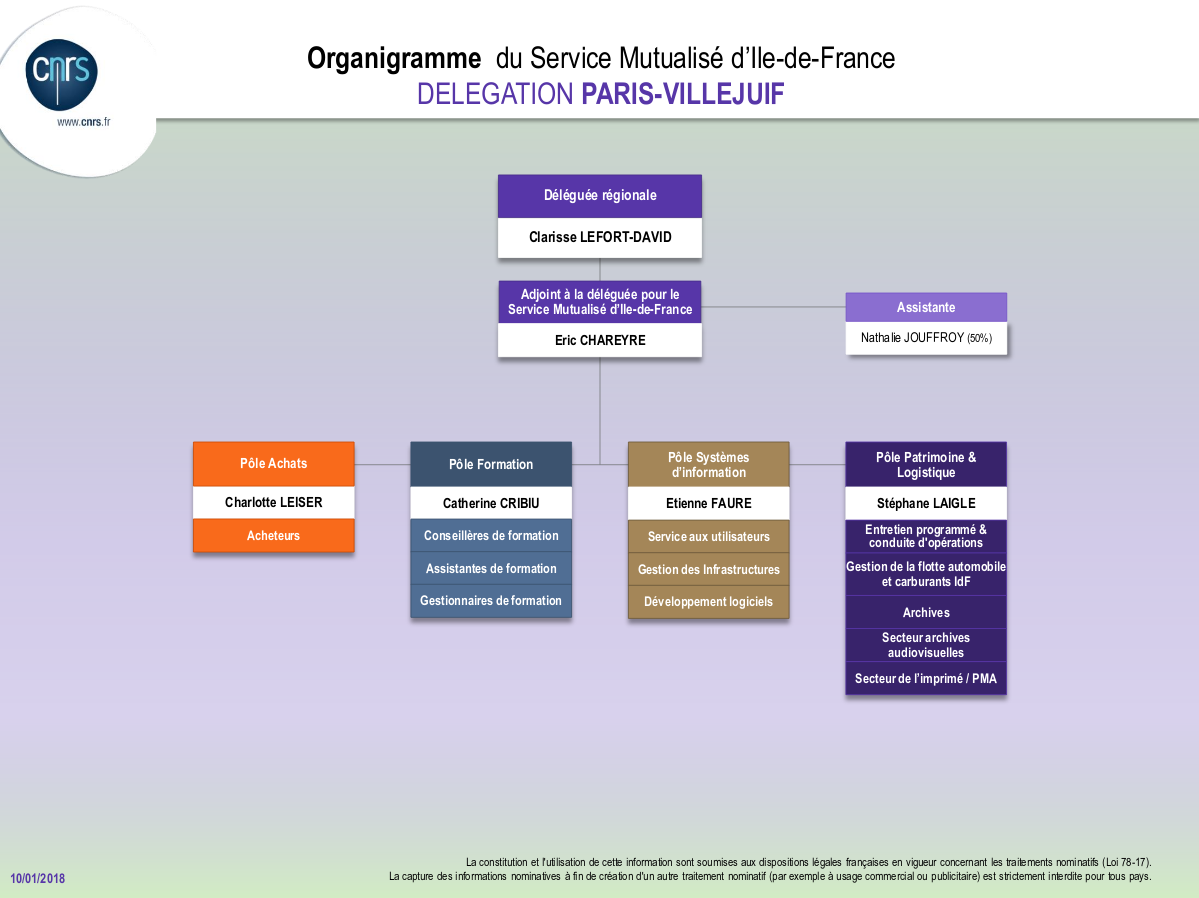
\includegraphics[width=15cm]{./images/ifsemorga.png}}

\subsection{Sources}
\begin{itemize}
    \item \url{http://www.cnrs.fr/}
    \item \url{https://www.dr1.cnrs.fr/spip.php?rubrique59}
    \item \url{https://fr.wikipedia.org/wiki/Centre_national_de_la_recherche_scientifique}
    \item \url{https://otrs.com/product-otrs/}
    \item \url{https://www.dr1.cnrs.fr/spip.php?article180}
    \item \url{https://blog.misterbean.fr/machine-cafe-entreprise}
    \item \url{https://www.quest.com/fr-fr/products/kace-systems-management-appliance/}
\end{itemize}
\newpage
\subsection{Attestation de fin de stage}
\newpage
\subsection{Ordre de mission}
Comme expliqué en partie 3.1.2, j'ai dû me déplacer sur le campus de Meudon. J'ai donc demandé un d'ordre de mission que voici :
\\
\\
\textit{
Bonjour,\\
Je soussigné Etienne FAURE, responsable du pôle SI de l’IFSeM, atteste que Théo \\PERESSE-GOURBIL actuellement stagiaire de 1ere année de l’ESIEE Paris effectuera un déplacement professionnel à la délégation Régionale du CNRS à Meudon (92) le jeudi 18 juillet 2019 pour la journée.
\medbreak
Pour faire valoir ce que de droit.
\smallbreak
Etienne FAURE}
\subsection{Remerciements}
A l'issue de ce stage, je tiens à remercier Mr Éric WIRTH et tous les professeurs de l'unité P\up{5} pour m'avoir permis de rédiger CVs et lettres de motivations ainsi que dans la recherche ce stage. 
\smallbreak
Je voudrais sincèrement remercier Mr Etienne FAURE, responsable du pôle SI de l'IFSeM qui fut aussi mon tuteur de stage pour avoir accepté de m'accueillir dans cette entreprise et de réaliser ce stage qui fut très formateur.
\smallbreak
Je souhaiterais aussi remercier tout l'IFSeM pour m'avoir rapidement intégré au sein du groupe, en particulier Baptiste BARAKOWSKY, Louis HERMEL et Vincent ROBERT qui m'ont accueilli dans leur bureau et avec qui j'ai passé ce mois. Ils ont su rendre ce stage intéressant et enrichissant d'un point de vu personnel et professionnel.

\end{document}